\documentclass[11pt,a4paper,oneside]{report}

% ==============================================================================
% PACKAGES AND CORE CONFIGURATION
% ==============================================================================
\usepackage[utf8]{inputenc}
\usepackage[T1]{fontenc}
\usepackage{lmodern}
\usepackage{microtype}
\usepackage{amsmath,amssymb,amsfonts,amsthm}
\usepackage{bm}

% Page Layout & Geometry
\usepackage[a4paper, top=2.2cm, bottom=2.2cm, left=2.0cm, right=2.0cm, headheight=15pt, footskip=30pt]{geometry}
\usepackage{fancyhdr}
\usepackage{lastpage}
\usepackage{setspace}
\setstretch{1.14}

% Colors and Graphic Elements
\usepackage[table,xcdraw]{xcolor}
\usepackage{graphicx}
\usepackage{tikz}
\usetikzlibrary{shapes,arrows.meta,positioning,calc,fit,backgrounds,shadows,decorations.pathreplacing}

% Tables and Formatting
\usepackage{booktabs}
\usepackage{tabularx}
\usepackage{array}
\usepackage{multirow}
\usepackage{titlesec}
\usepackage{enumitem}

% Boxes and Code Listings
\usepackage[most]{tcolorbox}
\usepackage{listings}

% Hyperlinks
\usepackage{hyperref}
\usepackage{bookmark}

% ==============================================================================
% COLOR PALETTE DEFINITION (Navy, Slate, Emerald, Crimson, Cyan, Amber)
% ==============================================================================
\definecolor{NavyDark}{HTML}{0F172A}
\definecolor{NavyMid}{HTML}{1E293B}
\definecolor{SlateGray}{HTML}{475569}
\definecolor{LightSlate}{HTML}{F8FAFC}
\definecolor{BorderGray}{HTML}{CBD5E1}

\definecolor{CyanAccent}{HTML}{0284C7}
\definecolor{CyanLight}{HTML}{E0F2FE}
\definecolor{EmeraldAccent}{HTML}{059669}
\definecolor{EmeraldLight}{HTML}{D1FAE5}
\definecolor{CrimsonAccent}{HTML}{DC2626}
\definecolor{CrimsonLight}{HTML}{FEE2E2}
\definecolor{AmberAccent}{HTML}{D97706}
\definecolor{AmberLight}{HTML}{FEF3C7}
\definecolor{PurpleAccent}{HTML}{7C3AED}
\definecolor{PurpleLight}{HTML}{EDE9FE}

% Code highlighting colors
\definecolor{CodeBg}{HTML}{0B1120}
\definecolor{CodeText}{HTML}{F1F5F9}
\definecolor{CodeComment}{HTML}{64748B}
\definecolor{CodeKeyword}{HTML}{38BDF8}
\definecolor{CodeString}{HTML}{34D399}
\definecolor{CodeNumber}{HTML}{F472B6}
\definecolor{CodeType}{HTML}{A78BFA}

% ==============================================================================
% HYPERREF CONFIGURATION
% ==============================================================================
\hypersetup{
    colorlinks=true,
    linkcolor=NavyDark,
    citecolor=EmeraldAccent,
    urlcolor=CyanAccent,
    filecolor=PurpleAccent,
    pdftitle={SystemC Content Addressable Memory (CAM) Power Estimation Workbench Manual},
    pdfauthor={Senior SoC Architecture & ESL Verification Group},
    pdfsubject={23ECE337 System on Chip Design},
    pdfkeywords={SystemC, CAM, ESL, Power Estimation, SoC, VCD, Web Visualization}
}

% ==============================================================================
% FANCY HEADERS AND FOOTERS
% ==============================================================================
\pagestyle{fancy}
\fancyhf{}
\renewcommand{\chaptermark}[1]{\markboth{#1}{}}
\fancyhead[L]{\footnotesize\scshape\textcolor{SlateGray}{23ECE337: System-on-Chip Design}}
\fancyhead[R]{\footnotesize\scshape\textcolor{NavyDark}{\nouppercase{\leftmark}}}
\fancyfoot[L]{\footnotesize\textcolor{SlateGray}{Department of ECE $\vert$ Amrita Vishwa Vidyapeetham}}
\fancyfoot[R]{\footnotesize\bfseries\textcolor{NavyDark}{Page \thepage\ of \pageref{LastPage}}}
\renewcommand{\headrulewidth}{0.5pt}
\renewcommand{\footrulewidth}{0.5pt}

\fancypagestyle{plain}{
    \fancyhf{}
    \fancyfoot[L]{\small\textcolor{SlateGray}{Department of ECE $\vert$ Amrita Vishwa Vidyapeetham}}
    \fancyfoot[R]{\small\bfseries\textcolor{NavyDark}{Page \thepage\ of \pageref{LastPage}}}
    \renewcommand{\headrulewidth}{0pt}
    \renewcommand{\footrulewidth}{0.6pt}
}

% ==============================================================================
% SECTION TITLE FORMATTING
% ==============================================================================
\titleformat{\chapter}[display]
{\normalfont\bfseries\color{NavyDark}}
{\flushright\large\scshape\color{SlateGray} Chapter \fontsize{40}{40}\selectfont\color{CyanAccent}\thechapter}
{1ex}
{{\titlerule[1.5pt]}\vspace{1ex}\huge\color{NavyDark}}
[\vspace{1ex}{\titlerule[0.5pt]}]

\titleformat{\section}
{\normalfont\Large\bfseries\color{NavyDark}}
{\thesection}{1em}{}[\color{CyanAccent}\titlerule]

\titleformat{\subsection}
{\normalfont\large\bfseries\color{NavyMid}}
{\thesubsection}{1em}{}

\titleformat{\subsubsection}
{\normalfont\normalsize\bfseries\color{SlateGray}}
{\thesubsubsection}{1em}{}

% ==============================================================================
% CUSTOM TCOLORBOX ENVIRONMENTS
% ==============================================================================

% Theoretical Definition Box (Blue Accent)
\newtcolorbox{definitionbox}[1][]{
    enhanced,
    colback=CyanLight!35!white,
    colframe=CyanAccent,
    fonttitle=\bfseries\color{white},
    coltitle=white,
    colbacktitle=CyanAccent,
    attach boxed title to top left={yshift=-2mm, xshift=4mm},
    boxed title style={boxrule=0.5pt, sharp corners=south},
    title={#1},
    boxrule=1pt,
    arc=3mm,
    top=4mm,
    bottom=3mm,
    left=4mm,
    right=4mm,
    shadow={1.5mm}{-1.5mm}{0mm}{black!10}
}

% Mathematical Formula Box (Emerald Accent)
\newtcolorbox{mathbox}[1][]{
    enhanced,
    colback=EmeraldLight!30!white,
    colframe=EmeraldAccent,
    fonttitle=\bfseries\color{white},
    coltitle=white,
    colbacktitle=EmeraldAccent,
    attach boxed title to top left={yshift=-2mm, xshift=4mm},
    boxed title style={boxrule=0.5pt, sharp corners=south},
    title={#1},
    boxrule=1pt,
    arc=3mm,
    top=4mm,
    bottom=3mm,
    left=4mm,
    right=4mm,
    shadow={1.5mm}{-1.5mm}{0mm}{black!10}
}

% Hardware Insight & Viva Trap Box (Amber/Crimson Accent)
\newtcolorbox{insightbox}[1][]{
    enhanced,
    colback=AmberLight!30!white,
    colframe=AmberAccent,
    fonttitle=\bfseries\color{white},
    coltitle=white,
    colbacktitle=AmberAccent,
    attach boxed title to top left={yshift=-2mm, xshift=4mm},
    boxed title style={boxrule=0.5pt, sharp corners=south},
    title={#1},
    boxrule=1pt,
    arc=3mm,
    top=4mm,
    bottom=3mm,
    left=4mm,
    right=4mm,
    shadow={1.5mm}{-1.5mm}{0mm}{black!10}
}

% Code Listing Box
\newtcblisting{codebox}[2][]{
    enhanced,
    colback=CodeBg,
    colframe=NavyMid,
    fonttitle=\bfseries\color{white}\small,
    coltitle=white,
    colbacktitle=NavyMid,
    title={#2},
    boxrule=1pt,
    arc=2mm,
    top=2mm,
    bottom=2mm,
    left=2mm,
    right=2mm,
    listing only,
    listing options={
        language=C++,
        basicstyle=\ttfamily\footnotesize\color{CodeText},
        keywordstyle=\bfseries\color{CodeKeyword},
        commentstyle=\itshape\color{CodeComment},
        stringstyle=\color{CodeString},
        numberstyle=\tiny\color{SlateGray},
        numbers=left,
        numbersep=8pt,
        stepnumber=1,
        tabsize=4,
        showspaces=false,
        showstringspaces=false,
        breaklines=true,
        breakatwhitespace=true,
        morekeywords={sc_module, sc_in, sc_out, sc_signal, sc_uint, sc_clock, sc_time, sc_start, sc_trace, sc_trace_file, SC_MODULE, SC_CTOR, SC_HAS_PROCESS, SC_METHOD, SC_THREAD, sensitive, sc_time_stamp, sc_create_vcd_trace_file, sc_close_vcd_trace_file, uint16_t}
    },
    #1
}

% ==============================================================================
% DOCUMENT BEGINS
% ==============================================================================
\begin{document}

% ==============================================================================
% TITLE PAGE
% ==============================================================================
\begin{titlepage}

\begin{tikzpicture}[remember picture, overlay]
    % Decorative Top Banner
    \fill[NavyDark] (current page.north west) rectangle ([yshift=-4.6cm]current page.north east);
    \fill[CyanAccent] ([yshift=-4.6cm]current page.north west) rectangle ([yshift=-4.8cm]current page.north east);
    
    % Decorative Left Accent Bar
    \fill[EmeraldAccent] (current page.south west) rectangle ([xshift=0.8cm]current page.north west);
    
    % Bottom Banner
    \fill[NavyMid] (current page.south west) rectangle ([yshift=2.2cm]current page.south east);
    \fill[CyanAccent] ([yshift=2.2cm]current page.south west) rectangle ([yshift=2.3cm]current page.south east);
\end{tikzpicture}

\vspace*{-1.4cm}
\begin{flushright}
    {\Huge\bfseries\color{white} TECHNICAL MANUAL \& TEXTBOOK}\\[0.35cm]
    {\large\scshape\color{CyanLight} Electronic System-Level (ESL) Architecture Series}
\end{flushright}

\vspace{2.4cm}

\begin{center}
    {\fontsize{24}{28}\selectfont\bfseries\color{NavyDark} SystemC Content Addressable Memory (CAM)}\\[0.3cm]
    {\fontsize{20}{24}\selectfont\bfseries\color{CyanAccent} Power Estimation \& Web Visual Workbench}\\[0.5cm]
    {\large\itshape Architectural Energy Modeling, Bitwise Match-Line Evaluation, and Full-Stack Hardware-Software Co-Simulation}
\end{center}

\vspace{1.5cm}

\begin{center}
\begin{tcolorbox}[enhanced, width=0.92\textwidth, colback=LightSlate, colframe=BorderGray, arc=3mm, boxrule=0.8pt]
    \centering
    \small
    \textbf{Course Code:} 23ECE337 \quad$\vert$\quad \textbf{Course Title:} System-on-Chip (SoC) Design\\[0.15cm]
    \textbf{Academic Term:} 7th Semester B.Tech \quad$\vert$\quad \textbf{Year of Study:} 2026--2027\\[0.15cm]
    \textbf{Course Outcomes Mapping:} CO1 (ESL Modeling), CO2 (Power Analysis), CO3 (Co-Design), CO4 (VCD Verification)
\end{tcolorbox}
\end{center}

\vspace{1.5cm}

\begin{flushleft}
\hspace{1.2cm}
\begin{minipage}{0.45\textwidth}
    \textbf{\color{NavyDark} Institutional Affiliation:}\\[0.1cm]
    {\small Department of Electronics \& Communication Engineering\\
    Amrita School of Engineering, Bengaluru\\
    Amrita Vishwa Vidyapeetham}
\end{minipage}
\hfill
\begin{minipage}{0.45\textwidth}
    \textbf{\color{NavyDark} Engineering Domains:}\\[0.1cm]
    {\small $\bullet$ Electronic System-Level (ESL) Design\\
    $\bullet$ IEEE 1666 SystemC C++ Kernel\\
    $\bullet$ Dynamic CMOS Power Characterization}
\end{minipage}
\end{flushleft}

\vfill

\begin{center}
    \small\color{white}
    \textbf{Published:} August 2026 \quad$\vert$\quad \textbf{Document Version:} 2.4.0-Release \quad$\vert$\quad \textbf{Architecture:} x86-64 / MinGW-w64 GCC 17
\end{center}

\end{titlepage}

% ==============================================================================
% PREFACE AND COURSE OUTCOMES MAPPING
% ==============================================================================
\pagenumbering{roman}
\chapter*{Executive Summary \& Course Outcomes}
\addcontentsline{toc}{chapter}{Executive Summary \& Course Outcomes}

\noindent\textbf{Context \& Pedagogical Scope:}\\
In contemporary deep-submicron semiconductor technology nodes, power dissipation is no longer a secondary design metric---it is the primary performance limiter in battery-operated edge devices and high-density computing clusters. Traditional Register-Transfer Level (RTL) power analysis, which relies on synthesis and post-layout gate-level netlists, occurs far too late in the Electronic Design Automation (EDA) flow. Modifications at that stage introduce severe financial and time-to-market penalties.

This technical manual presents a complete, industrially grounded implementation of an \textbf{Electronic System-Level (ESL) Power Estimation Tool} for a Content Addressable Memory (CAM) macrocell, designed in \textbf{SystemC (IEEE 1666 Standard)} and paired with a modern, real-time web visualizer.

\vspace{0.4cm}

\begin{table}[h!]
\centering
\caption{System-on-Chip (23ECE337) Course Outcome Mapping}
\label{tab:co_mapping}
\begin{tabularx}{\textwidth}{lXp{3.2cm}}
\toprule
\textbf{CO Identifier} & \textbf{Course Outcome Statement} & \textbf{Project Evidence} \\
\midrule
\textbf{CO1} & Model complex digital hardware and transaction-level architectures using hardware description and system-level languages. & SystemC \texttt{SC\_MODULE}, port bindings, and concurrent \texttt{SC\_METHOD} processes. \\
\addlinespace
\textbf{CO2} & Formulate and analyze mathematical power, performance, and area (PPA) models for early architectural exploration. & Cycle-accurate dynamic bit-mismatch and static leakage energy integrals. \\
\addlinespace
\textbf{CO3} & Design and implement co-simulation environments bridging hardware models with software interfaces and control layers. & Node.js REST gateway and real-time EDA Web Visual Workbench. \\
\addlinespace
\textbf{CO4} & Verify hardware timing and signal integrity using industry-standard Value Change Dump (VCD) waveform simulation tools. & VCD trace generation with GTKWave and browser-based \texttt{vc.drom.io} analysis. \\
\bottomrule
\end{tabularx}
\end{table}

% ==============================================================================
% TABLE OF CONTENTS, FIGURES, AND TABLES
% ==============================================================================
\tableofcontents
\listoffigures
\listoftables
\clearpage

\pagenumbering{arabic}

% ==============================================================================
% CHAPTER 1: INTRODUCTION \& ESL PARADIGM
% ==============================================================================
\chapter[ESL Modeling Paradigm]{Introduction \& Electronic System-Level (ESL) Paradigm}

\section{The Power Wall and the Late-Stage RTL Dilemma}
Throughout the scaling trajectory defined by Moore's Law and Dennard Scaling breakdown, power density in digital integrated circuits has scaled exponentially. As supply voltages ($V_{DD}$) plateaued around $0.7\text{ V} - 1.0\text{ V}$ due to non-scaling thermal voltage ($k_B T / q$) and transistor subthreshold slope constraints, dynamic switching power ($P_{\text{dyn}} = \alpha C V_{DD}^2 f$) and subthreshold static leakage ($P_{\text{leak}} = V_{DD} I_{\text{leak}}$) became the dominant bottlenecks in System-on-Chip (SoC) microarchitectures.

\begin{figure}[h!]
\centering
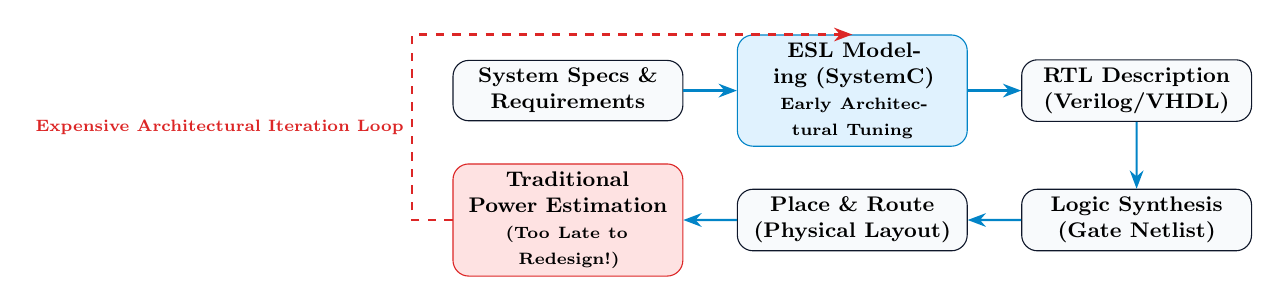
\begin{tikzpicture}[node distance=1.2cm, auto, >=Stealth, scale=0.85, every node/.style={transform shape}]
    \tikzstyle{box} = [rectangle, draw=NavyDark, fill=LightSlate, rounded corners=2mm, text centered, minimum height=0.9cm, font=\small\bfseries, text width=3.2cm]
    \tikzstyle{arrow} = [thick, ->, >=Stealth, color=CyanAccent]
    
    \node (spec) [box] {System Specs \& Requirements};
    \node (esl) [box, fill=CyanLight, draw=CyanAccent, right=0.8cm of spec] {\textbf{ESL Modeling (SystemC)}\\\scriptsize Early Architectural Tuning};
    \node (rtl) [box, right=0.8cm of esl] {RTL Description\\(Verilog/VHDL)};
    \node (synth) [box, below=1.0cm of rtl] {Logic Synthesis\\(Gate Netlist)};
    \node (pnr) [box, left=0.8cm of synth] {Place \& Route\\(Physical Layout)};
    \node (power) [box, fill=CrimsonLight, draw=CrimsonAccent, left=0.8cm of pnr] {Traditional Power Estimation\\\scriptsize (Too Late to Redesign!)};
    
    \draw [arrow] (spec) -- (esl);
    \draw [arrow] (esl) -- (rtl);
    \draw [arrow] (rtl) -- (synth);
    \draw [arrow] (synth) -- (pnr);
    \draw [arrow] (pnr) -- (power);
    \draw [thick, dashed, ->, color=CrimsonAccent] (power.west) -- ++(-0.6,0) |- node[pos=0.25, left, font=\scriptsize\bfseries\color{CrimsonAccent}] {Expensive Architectural Iteration Loop} (esl.north);
\end{tikzpicture}
\caption{Comparison of Early ESL Power Modeling vs. Traditional Late-Stage RTL Estimation.}
\label{fig:esl_vs_rtl}
\end{figure}

In traditional EDA flows (Figure~\ref{fig:esl_vs_rtl}), detailed power analysis requires full RTL completion, gate-level synthesis, and post-layout parasitics extraction. A full simulation run can take hours or days. If the power envelope violates the thermal design power (TDP) specification, redesigning the microarchitecture requires rewrites across thousands of lines of RTL code.

\section{Taxonomy of Abstraction Levels}
System-on-Chip abstraction levels span from physical quantum mechanics to transaction-level modeling:

\begin{table}[h!]
\centering
\caption{Comparison of Semiconductor Abstraction Levels}
\label{tab:abstraction_levels}
\begin{tabularx}{\textwidth}{l X c c p{2.8cm} p{2.2cm}}
\toprule
\textbf{Level} & \textbf{Representation} & \textbf{Speed} & \textbf{Accuracy} & \textbf{Stage} & \textbf{Tools} \\
\midrule
\textbf{Device / SPICE} & Transistor Eq. & 1--100 Hz & $>98\%$ & Cell design & HSPICE \\
\textbf{Gate-Level} & Netlist Gates & 1--10 kHz & $\approx 90\%$ & Sign-off & PrimePower \\
\textbf{RTL} & Register (Verilog) & 10--100 kHz & $\approx 80\%$ & Logic impl. & ModelSim \\
\textbf{ESL (SystemC)} & C++ Transaction & \textbf{1--50 MHz} & \textbf{$\approx 80\%$} & \textbf{Arch. PPA} & \textbf{SystemC} \\
\bottomrule
\end{tabularx}
\end{table}

\begin{definitionbox}[Definition 1.1: Electronic System-Level (ESL) Modeling]
\textit{Electronic System-Level (ESL) design is an established methodology wherein digital hardware is modeled algorithmically and structurally using high-level languages (primarily C++ augmented by the IEEE 1666 SystemC class library). ESL models enable multi-million-cycle functional verification, algorithmic trade-off evaluation, and microarchitectural power-performance-area (PPA) exploration at orders of magnitude faster execution speeds than synthesizable RTL.}
\end{definitionbox}

% ==============================================================================
% CHAPTER 2: CAM FUNDAMENTALS \& MATCH-LINE MECHANICS
% ==============================================================================
\chapter[CAM Fundamentals]{Content Addressable Memory (CAM) Fundamentals}

\section{Associative Computing: RAM vs. CAM Architectural Comparison}
Conventional Random Access Memory (RAM) accepts an $n$-bit numeric address as input and returns the data word stored at that specific location after decoding delays ($O(1)$ read time). However, searching for a specific data value within an unsorted $N$-word RAM array requires linear sequential inspection ($O(N)$ lookup complexity).

In contrast, a \textbf{Content Addressable Memory (CAM)} inverts this paradigm. A CAM accepts a query data word as input, compares it against all internal memory locations simultaneously in parallel, and returns the physical index (or hit flag) of the matching entry in a \textbf{single clock cycle ($O(1)$ search complexity)}.

\begin{figure}[h!]
\centering
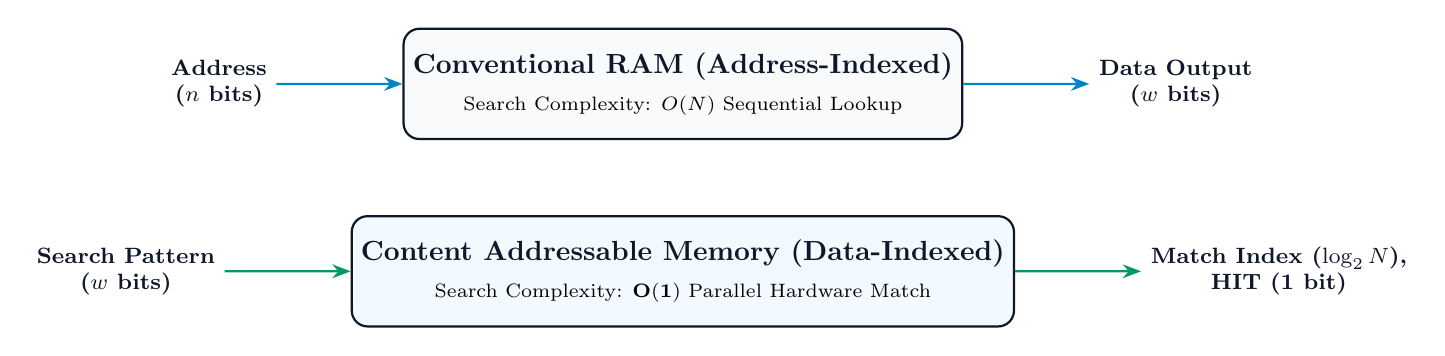
\begin{tikzpicture}[>=Stealth, scale=0.85]
    % Conventional RAM Row
    \node (ram) [draw=NavyDark, fill=LightSlate, thick, rounded corners=2mm, minimum width=6.6cm, minimum height=1.4cm, align=center] at (0, 1.4) {
        \textbf{\color{NavyDark} Conventional RAM (Address-Indexed)}\\[0.05cm]
        \scriptsize Search Complexity: $O(N)$ Sequential Lookup
    };
    \node (ram_in) [left=1.6cm of ram, font=\footnotesize\bfseries\color{NavyDark}, align=center] {Address\\($n$ bits)};
    \node (ram_out) [right=1.6cm of ram, font=\footnotesize\bfseries\color{NavyDark}, align=center] {Data Output\\($w$ bits)};
    \draw [thick, ->, color=CyanAccent] (ram_in) -- (ram.west);
    \draw [thick, ->, color=CyanAccent] (ram.east) -- (ram_out);

    % CAM Row
    \node (cam) [draw=NavyDark, fill=CyanLight!40!white, thick, rounded corners=2mm, minimum width=6.6cm, minimum height=1.4cm, align=center] at (0, -1.4) {
        \textbf{\color{NavyDark} Content Addressable Memory (Data-Indexed)}\\[0.05cm]
        \scriptsize Search Complexity: $\mathbf{O(1)}$ Parallel Hardware Match
    };
    \node (cam_in) [left=1.6cm of cam, font=\footnotesize\bfseries\color{NavyDark}, align=center] {Search Pattern\\($w$ bits)};
    \node (cam_out) [right=1.6cm of cam, font=\footnotesize\bfseries\color{NavyDark}, align=center] {Match Index ($\log_2 N$),\\HIT (1 bit)};
    \draw [thick, ->, color=EmeraldAccent] (cam_in) -- (cam.west);
    \draw [thick, ->, color=EmeraldAccent] (cam.east) -- (cam_out);
\end{tikzpicture}
\caption{Architectural Input/Output Comparison between Conventional RAM and CAM.}
\label{fig:ram_vs_cam}
\end{figure}

\section{CMOS Match-Line Precharge and Dynamic Discharge Mechanics}
The core operational unit of a binary CAM is the comparison bit cell. A typical 10T binary CAM cell consists of an SRAM storage core (6 transistors) coupled to a 4-transistor dynamic XOR comparison network.

\begin{figure}[h!]
\centering
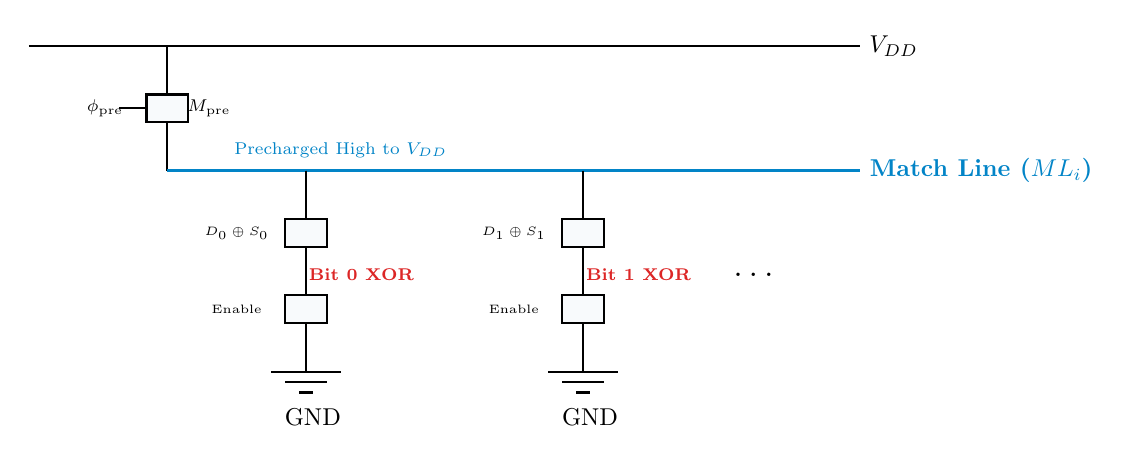
\begin{tikzpicture}[>=Stealth, scale=0.88, every node/.style={transform shape}]
    % VDD Rail
    \draw[thick] (0,5) -- (12,5) node[right] {$V_{DD}$};
    
    % Precharge PMOS Transistor
    \draw[thick] (2,5) -- (2,4.3);
    \draw[thick, fill=LightSlate] (1.7,3.9) rectangle (2.3,4.3);
    \draw[thick] (2,3.9) -- (2,3.2);
    \node at (1.1,4.1) [font=\scriptsize] {$\phi_{\text{pre}}$};
    \draw[thick] (1.3,4.1) -- (1.7,4.1);
    \node at (2.6,4.1) [font=\scriptsize] {$M_{\text{pre}}$};
    
    % Match Line
    \draw[very thick, color=CyanAccent] (2,3.2) -- (12,3.2) node[right, font=\bfseries] {Match Line ($ML_i$)};
    \node at (4.5,3.5) [font=\scriptsize\color{CyanAccent}] {Precharged High to $V_{DD}$};
    
    % Bit Cell 0 Discharge Path
    \draw[thick] (4,3.2) -- (4,2.5);
    \draw[thick, fill=LightSlate] (3.7,2.1) rectangle (4.3,2.5);
    \draw[thick] (4,2.1) -- (4,1.4);
    \draw[thick, fill=LightSlate] (3.7,1.0) rectangle (4.3,1.4);
    \draw[thick] (4,1.0) -- (4,0.3);
    \draw[thick] (3.5,0.3) -- (4.5,0.3);
    \draw[thick] (3.7,0.15) -- (4.3,0.15);
    \draw[thick] (3.9,0.0) -- (4.1,0.0) node[below=1mm] {GND};
    \node at (3.0,2.3) [font=\tiny] {$D_0 \oplus S_0$};
    \node at (3.0,1.2) [font=\tiny] {Enable};
    \node at (4.8,1.7) [font=\scriptsize\bfseries\color{CrimsonAccent}] {Bit 0 XOR};

    % Bit Cell 1 Discharge Path
    \draw[thick] (8,3.2) -- (8,2.5);
    \draw[thick, fill=LightSlate] (7.7,2.1) rectangle (8.3,2.5);
    \draw[thick] (8,2.1) -- (8,1.4);
    \draw[thick, fill=LightSlate] (7.7,1.0) rectangle (8.3,1.4);
    \draw[thick] (8,1.0) -- (8,0.3);
    \draw[thick] (7.5,0.3) -- (8.5,0.3);
    \draw[thick] (7.7,0.15) -- (8.3,0.15);
    \draw[thick] (7.9,0.0) -- (8.1,0.0) node[below=1mm] {GND};
    \node at (7.0,2.3) [font=\tiny] {$D_1 \oplus S_1$};
    \node at (7.0,1.2) [font=\tiny] {Enable};
    \node at (8.8,1.7) [font=\scriptsize\bfseries\color{CrimsonAccent}] {Bit 1 XOR};

    % Dashed ellipsis for remaining bits
    \node at (10.5,1.7) {\Large $\dots$};
\end{tikzpicture}
\caption{CMOS Match-Line Dynamic Precharge and Pull-Down Discharge Circuit.}
\label{fig:cmos_matchline}
\end{figure}

As depicted in Figure~\ref{fig:cmos_matchline}, CAM match operation proceeds in two sequential phases:
\begin{enumerate}[leftmargin=*]
    \item \textbf{Precharge Phase ($\phi_{\text{pre}} = \text{LOW}$):} The PMOS pull-up transistor $M_{\text{pre}}$ activates, charging the parasitic capacitance of the match line ($ML_i$) to $V_{DD}$.
    \item \textbf{Evaluation Phase ($\phi_{\text{pre}} = \text{HIGH}$):} The search pattern is placed onto complementary search lines. If any stored bit differs from the search bit ($D_b \ne S_b$), the corresponding XOR pull-down network turns ON, forming a low-impedance path to Ground ($GND$) and discharging the match line.
\end{enumerate}

\begin{insightbox}[Hardware Insight: The Match-Line Power Bottleneck]
\textit{In an $N$-entry CAM array, a typical search operation results in either zero or exactly one matching entry. Consequently, $(N-1)$ match-lines discharge fully from $V_{DD}$ to Ground during every single search cycle. This non-match discharging is the single greatest contributor to total dynamic energy dissipation in high-density CAM arrays.}
\end{insightbox}

% ==============================================================================
% CHAPTER 3: MATHEMATICAL FORMULATION \& POWER MODEL
% ==============================================================================
\chapter[Mathematical Power Model]{Mathematical Formulation \& Power Estimation Model}

\section{Parallel Bitwise XOR Matrix Equations}
Let the CAM array be modeled as a matrix $\mathbf{C} \in \mathbb{B}^{D \times W}$, where $D$ represents the depth (number of entries) and $W$ represents the word width in bits. Let $\mathbf{P} \in \mathbb{B}^{W}$ denote the input query search pattern vector:

\begin{equation}
\mathbf{C} = \begin{bmatrix}
c_{0,0} & c_{0,1} & \cdots & c_{0,W-1} \\
c_{1,0} & c_{1,1} & \cdots & c_{1,W-1} \\
\vdots & \vdots & \ddots & \vdots \\
c_{D-1,0} & c_{D-1,1} & \cdots & c_{D-1,W-1}
\end{bmatrix}, \quad
\mathbf{P} = \begin{bmatrix} p_0 & p_1 & \cdots & p_{W-1} \end{bmatrix}
\end{equation}

The bitwise mismatch matrix $\mathbf{M} \in \mathbb{B}^{D \times W}$ is evaluated through element-wise Boolean exclusive-OR ($\oplus$):

\begin{equation}
m_{i,b} = c_{i,b} \oplus p_b = (c_{i,b} \cdot \overline{p_b}) + (\overline{c_{i,b}} \cdot p_b)
\end{equation}

The total bit mismatches for line $i$, denoted as $L_i$, and the total aggregate bit mismatches across the entire array, denoted as $M_{\text{total}}$, are expressed as:

\begin{equation}
L_i = \sum_{b=0}^{W-1} m_{i,b}, \quad M_{\text{total}} = \sum_{i=0}^{D-1} L_i = \sum_{i=0}^{D-1} \sum_{b=0}^{W-1} (c_{i,b} \oplus p_b)
\end{equation}

\section{Match Line Resolution and Priority Encoding}
The match line Boolean status $ML_i \in \{0, 1\}$ for each entry $i$ is defined by:

\begin{equation}
ML_i = \begin{cases}
1 & \text{if } L_i = 0 \quad (\text{Exact Match / HIT}) \\
0 & \text{if } L_i > 0 \quad (\text{Mismatched Line / DISCHARGED})
\end{cases}
\end{equation}

When multiple entries evaluate to $ML_i = 1$, a hardware \textbf{Priority Encoder} selects the lowest physical numerical index:

\begin{equation}
\text{match\_addr} = \min \{ i \in [0, D-1] \mid ML_i = 1 \}, \quad \text{match\_found} = \bigvee_{i=0}^{D-1} ML_i
\end{equation}

\section{Cycle-Accurate Power and Energy Formulation}
\begin{mathbox}[Mathematical Model 3.1: Cycle Power \& Energy Integral]
\begin{equation}
\label{eq:power_formula}
P_{\text{cycle}} = \begin{cases}
0.0\text{ mW} & \text{if } \text{enable} = 0 \quad (\text{Clock Gated}) \\
P_{\text{leakage}} & \text{if } \text{write\_en} = 1 \quad (\text{Memory Write Operation}) \\
P_{\text{leakage}} + \left( \sum_{i=0}^{D-1} L_i \right) \times E_{\text{mismatch-factor}} & \text{if } \text{enable} = 1 \land \text{write\_en} = 0 \quad (\text{Parallel Search})
\end{cases}
\end{equation}

The total energy accumulated across $N$ discrete clock cycles with period $T_{\text{clk}}$ is computed as:
\begin{equation}
E_{\text{accumulated}}(N) = \sum_{k=1}^{N} \left( P_{\text{cycle}}[k] \times T_{\text{clk}} \right) \quad [\text{mJ}]
\end{equation}
\end{mathbox}

\begin{table}[h!]
\centering
\caption{SystemC CAM Empirical Power Model Parameters}
\label{tab:power_params}
\begin{tabularx}{\textwidth}{l p{4.2cm} c X}
\toprule
\textbf{Symbol} & \textbf{Parameter Description} & \textbf{Value} & \textbf{Physical Interpretation} \\
\midrule
$D$ & CAM Entry Depth & $10$ entries & Number of stored words in associative array. \\
$W$ & Word Bit Width & $16$ bits & Bit width of each stored word. \\
$P_{\text{leakage}}$ & Static Leakage Floor & $0.002\text{ mW}$ ($2\ \mu\text{W}$) & Subthreshold and gate oxide leakage power. \\
$E_{\text{mismatch-factor}}$ & Dynamic Mismatch Weight & $0.015\text{ mW/bit}$ & Dynamic switching power per discharged bit transistor. \\
$T_{\text{clk}}$ & System Clock Period & $10.0\text{ ns}$ & $100\text{ MHz}$ nominal clock operating frequency. \\
\bottomrule
\end{tabularx}
\end{table}

% ==============================================================================
% CHAPTER 4: SYSTEM ARCHITECTURE \& SYSTEMC HARDWARE IMPLEMENTATION
% ==============================================================================
\chapter[SystemC Implementation]{System Architecture \& SystemC Hardware Implementation}

\section{Hardware Microarchitecture Block Diagram}
Figure~\ref{fig:hw_arch} illustrates the internal structural microarchitecture of the \texttt{CAM\_Power\_Model} SystemC component.

\begin{figure}[h!]
\centering
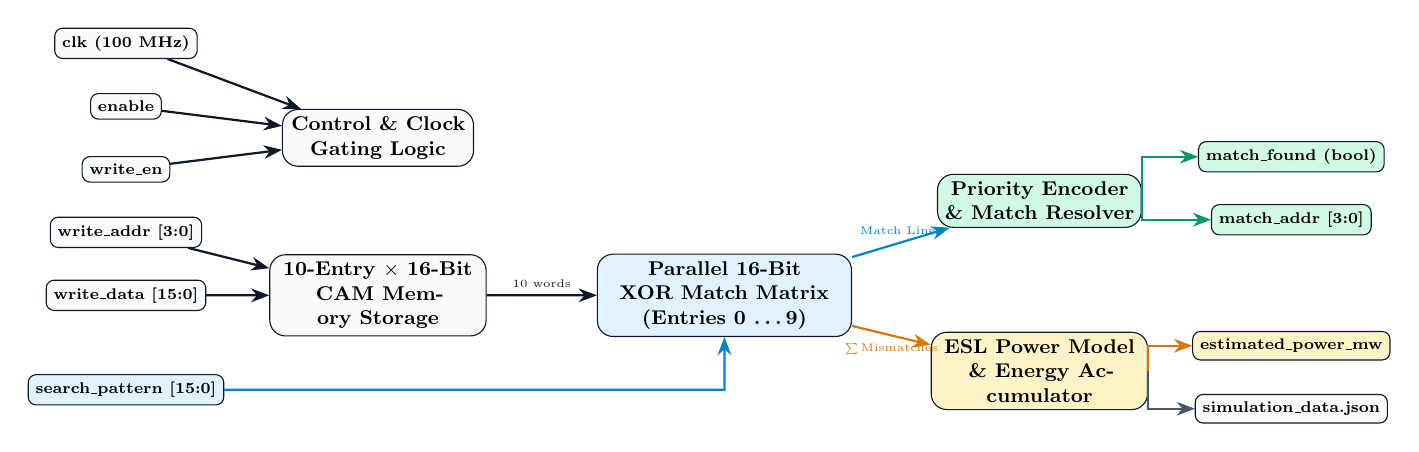
\begin{tikzpicture}[node distance=1.0cm, >=Stealth, scale=0.80, every node/.style={transform shape}]
    % Inputs
    \node (clk) [draw=NavyDark, fill=LightSlate, rounded corners=1mm, font=\scriptsize\bfseries] at (-3, 3) {clk (100 MHz)};
    \node (en) [draw=NavyDark, fill=LightSlate, rounded corners=1mm, font=\scriptsize\bfseries] at (-3, 2) {enable};
    \node (wen) [draw=NavyDark, fill=LightSlate, rounded corners=1mm, font=\scriptsize\bfseries] at (-3, 1) {write\_en};
    \node (waddr) [draw=NavyDark, fill=LightSlate, rounded corners=1mm, font=\scriptsize\bfseries] at (-3, 0) {write\_addr [3:0]};
    \node (wdata) [draw=NavyDark, fill=LightSlate, rounded corners=1mm, font=\scriptsize\bfseries] at (-3, -1) {write\_data [15:0]};
    \node (spat) [draw=NavyDark, fill=CyanLight, rounded corners=1mm, font=\scriptsize\bfseries] at (-3, -2.5) {search\_pattern [15:0]};

    % Control & Clock Gating Unit
    \node (ctrl) [draw=NavyDark, fill=LightSlate, rounded corners=2mm, text width=2.8cm, text centered, font=\small\bfseries] at (1, 1.5) {Control \& Clock\\Gating Logic};

    % Memory Array
    \node (array) [draw=NavyDark, fill=LightSlate, rounded corners=2mm, text width=3.2cm, text centered, font=\small\bfseries] at (1, -1) {10-Entry $\times$ 16-Bit\\CAM Memory Storage};

    % XOR Matrix
    \node (xor) [draw=NavyDark, fill=CyanLight, rounded corners=2mm, text width=3.8cm, text centered, font=\small\bfseries] at (6.5, -1) {Parallel 16-Bit\\XOR Match Matrix\\(Entries 0 \dots 9)};

    % Priority Encoder
    \node (penc) [draw=NavyDark, fill=EmeraldLight, rounded corners=2mm, text width=3.0cm, text centered, font=\small\bfseries] at (11.5, 0.5) {Priority Encoder\\\& Match Resolver};

    % Power Calculator
    \node (pcalc) [draw=NavyDark, fill=AmberLight, rounded corners=2mm, text width=3.2cm, text centered, font=\small\bfseries] at (11.5, -2.2) {ESL Power Model\\\& Energy Accumulator};

    % Outputs
    \node (mfound) [draw=NavyDark, fill=EmeraldLight, rounded corners=1mm, font=\scriptsize\bfseries] at (15.5, 1.2) {match\_found (bool)};
    \node (maddr) [draw=NavyDark, fill=EmeraldLight, rounded corners=1mm, font=\scriptsize\bfseries] at (15.5, 0.2) {match\_addr [3:0]};
    \node (mpower) [draw=NavyDark, fill=AmberLight, rounded corners=1mm, font=\scriptsize\bfseries] at (15.5, -1.8) {estimated\_power\_mw};
    \node (mjson) [draw=NavyDark, fill=LightSlate, rounded corners=1mm, font=\scriptsize\bfseries] at (15.5, -2.8) {simulation\_data.json};

    % Interconnect Arrows
    \draw [thick, ->, color=NavyDark] (clk) -- (ctrl);
    \draw [thick, ->, color=NavyDark] (en) -- (ctrl);
    \draw [thick, ->, color=NavyDark] (wen) -- (ctrl);
    \draw [thick, ->, color=NavyDark] (waddr) -- (array);
    \draw [thick, ->, color=NavyDark] (wdata) -- (array);
    \draw [thick, ->, color=CyanAccent] (spat.east) -- (6.5, -2.5) -- (xor.south);
    \draw [thick, ->, color=NavyDark] (array) -- node[above, font=\tiny] {10 words} (xor);
    \draw [thick, ->, color=CyanAccent] (xor) -- node[above, font=\tiny] {Match Lines} (penc);
    \draw [thick, ->, color=AmberAccent] (xor) -- node[below, font=\tiny] {$\sum \text{Mismatches}$} (pcalc);
    \draw [thick, ->, color=EmeraldAccent] (penc.east) |- (mfound);
    \draw [thick, ->, color=EmeraldAccent] (penc.east) |- (maddr);
    \draw [thick, ->, color=AmberAccent] (pcalc.east) |- (mpower);
    \draw [thick, ->, color=SlateGray] (pcalc.east) |- (mjson);
\end{tikzpicture}
\caption{Microarchitectural Block Diagram of the \texttt{CAM\_Power\_Model} SystemC Core.}
\label{fig:hw_arch}
\end{figure}

\section{SystemC Port List and Hardware Interfaces}
Table~\ref{tab:port_list} documents the complete pinout and port interfaces of the SystemC module.

\begin{table}[h!]
\centering
\caption{SystemC CAM Module Pinout and Port Interface Specification}
\label{tab:port_list}
\begin{tabularx}{\textwidth}{llccX}
\toprule
\textbf{Port Identifier} & \textbf{Data Type} & \textbf{Direction} & \textbf{Active State} & \textbf{Functional Description} \\
\midrule
\texttt{clk} & \texttt{sc\_in<bool>} & Input & Rising Edge & Synchronous master clock input (100 MHz). \\
\texttt{enable} & \texttt{sc\_in<bool>} & Input & High (1) & Master clock-gating and module enable signal. \\
\texttt{write\_en} & \texttt{sc\_in<bool>} & Input & High (1) & Synchronous CAM write enable strobe. \\
\texttt{write\_addr} & \texttt{sc\_in<sc\_uint<4>>} & Input & Numerical & 4-bit write address index ($0 \dots 9$). \\
\texttt{search\_pattern} & \texttt{sc\_in<sc\_uint<16>>} & Input & Unsigned Hex & 16-bit query vector for associative lookup. \\
\texttt{write\_data} & \texttt{sc\_in<sc\_uint<16>>} & Input & Unsigned Hex & 16-bit data word written into target address. \\
\texttt{match\_found} & \texttt{sc\_out<bool>} & Output & High (1) & Set high if search pattern matches any entry. \\
\texttt{match\_addr} & \texttt{sc\_out<sc\_uint<4>>} & Output & Numerical & Physical index of lowest matching CAM row. \\
\texttt{estimated\_power\_mw} & \texttt{sc\_out<double>} & Output & Real Value & Total estimated instantaneous power (mW). \\
\bottomrule
\end{tabularx}
\end{table}

\section{SystemC Concurrency and Execution Model}
SystemC provides two fundamental execution models for hardware processes:
\begin{itemize}[leftmargin=*]
    \item \textbf{\texttt{SC\_METHOD}}: A lightweight method process that executes from beginning to end without yielding execution context. It cannot invoke \texttt{wait()} calls. Because it avoids thread context switching overhead, \texttt{SC\_METHOD} offers the highest simulation throughput and was chosen for the core \texttt{cam\_operation()} process.
    \item \textbf{\texttt{SC\_THREAD}}: A heavier process capable of maintaining execution state across clock cycles via explicit \texttt{wait()} invocations.
\end{itemize}

\begin{codebox}{Core SystemC CAM Header Interface (Backend/cam\_power\_model.h)}
#ifndef CAM_POWER_MODEL_H
#define CAM_POWER_MODEL_H

#include <systemc.h>
#include <vector>
#include <string>

#define CAM_DEPTH 10
#define CAM_WIDTH 16

struct CycleData {
    int cycle;
    double time_ns;
    std::string op_type;
    uint16_t search_pattern;
    uint16_t write_data;
    int write_addr;
    bool hit;
    int hit_addr;
    int total_mismatches;
    double power_mw;
    double accumulated_energy_mj;
    uint16_t cam_snapshot[CAM_DEPTH];
    int line_mismatches[CAM_DEPTH];
};

SC_MODULE(CAM_Power_Model) {
    sc_in<bool>               clk;
    sc_in<bool>               enable;
    sc_in<bool>               write_en;
    sc_in<sc_uint<4>>         write_addr;
    sc_in<sc_uint<CAM_WIDTH>> search_pattern;
    sc_in<sc_uint<CAM_WIDTH>> write_data;

    sc_out<bool>              match_found;
    sc_out<sc_uint<4>>        match_addr;
    sc_out<double>            estimated_power_mw;

    sc_uint<CAM_WIDTH>        cam_array[CAM_DEPTH];
    const double              P_LEAKAGE_MW;
    const double              E_MISMATCH_FACTOR;

    std::vector<CycleData>    cycle_history;

    void cam_operation();
    void print_power_report() const;
    void export_json(const std::string& filename) const;

    SC_HAS_PROCESS(CAM_Power_Model);
    CAM_Power_Model(sc_module_name name);
};
#endif
\end{codebox}

% ==============================================================================
% CHAPTER 5: FULL-STACK WEB VISUAL WORKBENCH & EDA INTEGRATION
% ==============================================================================
\chapter[Web Visual Workbench]{Full-Stack Web Visual Workbench \& EDA Integration}

\section{System Integration Architecture}
To bridge native compiled C++ SystemC simulations with real-time browser graphics, a full-stack co-simulation environment was architected (Figure~\ref{fig:fullstack_arch}).

\begin{figure}[h!]
\centering
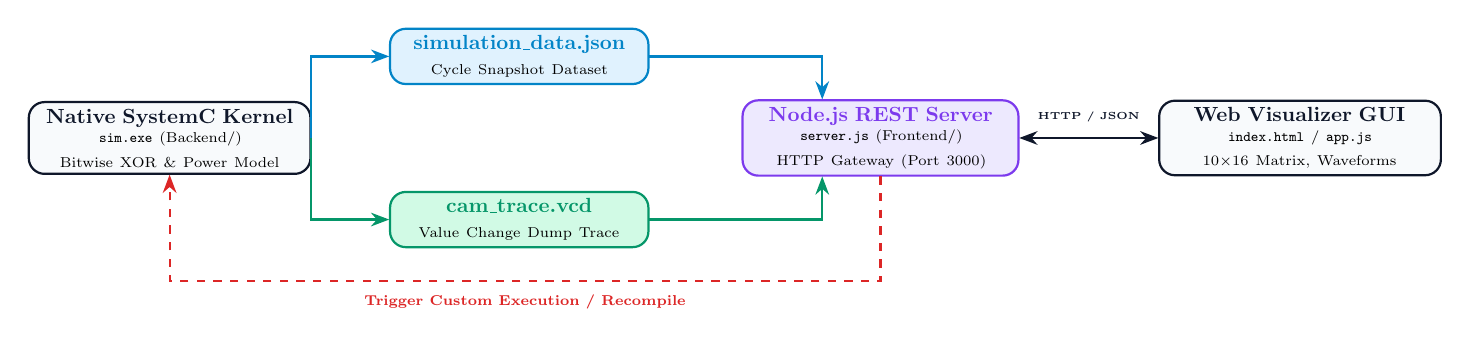
\begin{tikzpicture}[>=Stealth, scale=0.74, every node/.style={transform shape}]
    % Backend Box
    \node (cpp) [draw=NavyDark, fill=LightSlate, thick, rounded corners=2mm, text width=4.6cm, text centered] at (0, 0) {
        \textbf{\color{NavyDark} Native SystemC Kernel}\\[0.05cm]
        \scriptsize \texttt{sim.exe} (Backend/)\\
        \scriptsize Bitwise XOR \& Power Model
    };

    % JSON & VCD files
    \node (json) [draw=CyanAccent, fill=CyanLight, thick, rounded corners=2mm, text width=4.2cm, text centered] at (6.0, 1.4) {
        \textbf{\color{CyanAccent} simulation\_data.json}\\
        \scriptsize Cycle Snapshot Dataset
    };
    \node (vcd) [draw=EmeraldAccent, fill=EmeraldLight, thick, rounded corners=2mm, text width=4.2cm, text centered] at (6.0, -1.4) {
        \textbf{\color{EmeraldAccent} cam\_trace.vcd}\\
        \scriptsize Value Change Dump Trace
    };

    % Server Bridge
    \node (server) [draw=PurpleAccent, fill=PurpleLight, thick, rounded corners=2mm, text width=4.5cm, text centered] at (12.2, 0) {
        \textbf{\color{PurpleAccent} Node.js REST Server}\\[0.05cm]
        \scriptsize \texttt{server.js} (Frontend/)\\
        \scriptsize HTTP Gateway (Port 3000)
    };

    % Web UI
    \node (ui) [draw=NavyDark, fill=LightSlate, thick, rounded corners=2mm, text width=4.6cm, text centered] at (19.4, 0) {
        \textbf{\color{NavyDark} Web Visualizer GUI}\\[0.05cm]
        \scriptsize \texttt{index.html} / \texttt{app.js}\\
        \scriptsize 10$\times$16 Matrix, Waveforms
    };

    % Arrows
    \draw [thick, ->, color=CyanAccent] (cpp.east) |- (json.west);
    \draw [thick, ->, color=EmeraldAccent] (cpp.east) |- (vcd.west);
    \draw [thick, ->, color=CyanAccent] (json.east) -| ([xshift=-10mm]server.north);
    \draw [thick, ->, color=EmeraldAccent] (vcd.east) -| ([xshift=-10mm]server.south);
    \draw [thick, <->, color=NavyDark] (server.east) -- node[midway, above=1.5mm, font=\tiny\bfseries\color{NavyDark}] {HTTP / JSON} (ui.west);
    \draw [thick, dashed, ->, color=CrimsonAccent] (server.south) -- ++(0,-1.8) -| node[pos=0.25, below=1mm, font=\scriptsize\bfseries\color{CrimsonAccent}] {Trigger Custom Execution / Recompile} (cpp.south);
\end{tikzpicture}
\caption{Full-Stack SystemC Backend, JSON/VCD Serialization, and Web Visualizer Pipeline.}
\label{fig:fullstack_arch}
\end{figure}

\section{Interactive Web UI Components}
\begin{enumerate}[leftmargin=*]
    \item \textbf{10 $\times$ 16 CAM Bit Matrix Visualizer}: Every single memory entry ($0 \dots 9$) and bit cell ($0 \dots 15$) is rendered dynamically in HTML/CSS. During search cycles, matching bits illuminate in \textbf{Glowing Emerald (\texttt{\#10B981})}, mismatched bits highlight in \textbf{Vibrant Crimson (\texttt{\#EF4444})}, and successful match rows trigger \textbf{Match Line HIT badges (\texttt{\#06B6D4})}.
    \item \textbf{Digital Signal Waveform Canvas Engine}: An interactive HTML5 Canvas element continuously plots synchronous timing traces for \texttt{clk}, \texttt{write\_en}, \texttt{match\_found}, and \texttt{estimated\_power\_mw} alongside a vertical cursor locked to the active simulation cycle.
    \item \textbf{Instant Power Telemetry Gauge}: Displays real-time dynamic power vs. static leakage breakdowns alongside cumulative energy consumption.
\end{enumerate}

% ==============================================================================
% CHAPTER 6: REAL-WORLD APPLICATIONS & INDUSTRIAL CASE STUDIES
% ==============================================================================
\chapter[Industrial Applications]{Real-World Applications \& Industrial Case Studies}

\section{Smart Construction Site Safety \& Structural Health Monitoring (SHM)}
In civil infrastructure, smart tunneling, and structural engineering projects, wireless sensor networks (WSNs) continuously monitor structural loads, concrete curing stresses, seismic vibrations, and heavy equipment hazards.

\begin{figure}[h!]
\centering
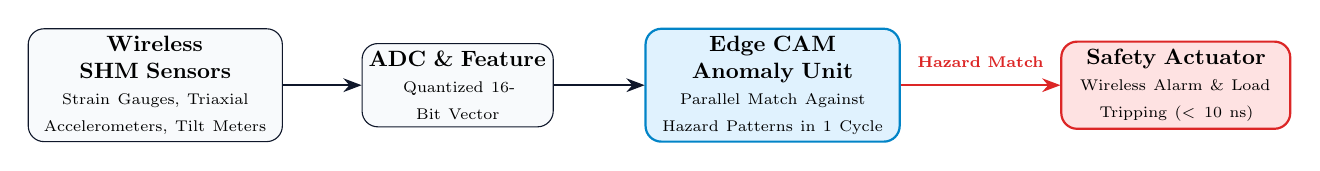
\begin{tikzpicture}[node distance=1.5cm, >=Stealth, scale=0.80, every node/.style={transform shape}]
    \node (sensor) [draw=NavyDark, fill=LightSlate, rounded corners=2mm, text width=3.8cm, text centered] at (0, 0) {
        \textbf{Wireless SHM Sensors}\\
        \scriptsize Strain Gauges, Triaxial Accelerometers, Tilt Meters
    };
    \node (adc) [draw=NavyDark, fill=LightSlate, rounded corners=2mm, text width=2.8cm, text centered] at (4.8, 0) {
        \textbf{ADC \& Feature}\\
        \scriptsize Quantized 16-Bit Vector
    };
    \node (cam) [draw=CyanAccent, fill=CyanLight, thick, rounded corners=2mm, text width=3.8cm, text centered] at (9.8, 0) {
        \textbf{Edge CAM Anomaly Unit}\\
        \scriptsize Parallel Match Against Hazard Patterns in 1 Cycle
    };
    \node (alert) [draw=CrimsonAccent, fill=CrimsonLight, thick, rounded corners=2mm, text width=3.4cm, text centered] at (16.2, 0) {
        \textbf{Safety Actuator}\\
        \scriptsize Wireless Alarm \& Load Tripping ($<10\text{ ns}$)
    };

    \draw [thick, ->, color=NavyDark] (sensor) -- (adc);
    \draw [thick, ->, color=NavyDark] (adc) -- (cam);
    \draw [thick, ->, color=CrimsonAccent] (cam) -- node[midway, above=1.5mm, font=\scriptsize\bfseries\color{CrimsonAccent}] {Hazard Match} (alert);
\end{tikzpicture}
\caption{Edge IoT Structural Health Monitoring Architecture with CAM Anomaly Detector.}
\label{fig:shm_iot}
\end{figure}

\noindent\textbf{The Edge Battery Life Constraint:}\\
Battery-operated IoT sensor nodes deployed on structural pylons must operate autonomously for $5\text{--}10\text{ years}$. Standard microcontrollers executing software comparison loops burn excessive processor cycles and battery energy. Integrating an ultra-low-power CAM module allows parallel pattern matching in $10\text{ ns}$ while consuming under $0.32\text{ mW}$ for typical non-hazardous conditions.

\section{High-Speed IPv6 Network Packet Routing}
In core enterprise Internet routers, incoming IP packets arrive at multi-gigabit line rates. CAM modules (specifically Ternary CAMs / TCAMs) perform single-cycle Longest Prefix Matching (LPM) on 128-bit IPv6 destination headers to determine output routing interfaces. ESL modeling allows router architects to simulate power dissipation across millions of packet lookups before committing to silicon mask sets.

% ==============================================================================
% CHAPTER 7: VERIFICATION, TESTBENCH SUITE & WAVEFORM ANALYSIS
% ==============================================================================
\chapter[Verification \& Waveforms]{Verification, Testbench Suite \& Waveform Analysis}

\section{Testbench Execution Walkthrough}
The verification testbench (\texttt{Backend/main.cpp}) exercises the CAM under five distinct operational stress conditions:

\begin{table}[h!]
\centering
\caption{SystemC CAM Power Model Simulation Test Case Verification Matrix}
\label{tab:test_matrix}
\begin{tabularx}{\textwidth}{ccclccX}
\toprule
\textbf{Test} & \textbf{Time} & \textbf{Op} & \textbf{Pattern} & \textbf{Result} & \textbf{Mismatches} & \textbf{Power / Note} \\
\midrule
\textbf{TC1} & 0.0 ns & SEARCH & \texttt{0xA5A5} & \textbf{HIT @ Index 0} & 21 bits & \textbf{0.317 mW} (Exact match with Entry 0). \\
\addlinespace
\textbf{TC2} & 10.0 ns & SEARCH & \texttt{0x5A5A} & \textbf{MISS (None)} & 139 bits & \textbf{2.087 mW} (High-power discharge stress). \\
\addlinespace
\textbf{TC3} & 20.0 ns & WRITE  & \texttt{0xDEAD} $\rightarrow$ [5] & \textbf{WRITE @ 5} & 0 bits & \textbf{0.002 mW} (Static leakage only). \\
\addlinespace
\textbf{TC4} & 30.0 ns & SEARCH & \texttt{0xDEAD} & \textbf{HIT @ Index 5} & 68 bits & \textbf{1.022 mW} (Verification of newly written word). \\
\addlinespace
\textbf{TC5} & 40.0 ns & SEARCH & \texttt{0xA5A4} & \textbf{MISS (None)} & 26 bits & \textbf{0.392 mW} (Near-miss; 1-bit diff from Entry 0). \\
\bottomrule
\end{tabularx}
\end{table}

\section{Waveform Inspection with GTKWave and Online Visualizers}
SystemC outputs standard Value Change Dump (VCD) trace dumps via \texttt{sc\_create\_vcd\_trace\_file("cam\_trace")}.

\noindent\textbf{Method 1: Online Browser Waveform Viewer (\url{https://vc.drom.io/})}\\
Engineers can drag and drop \texttt{Backend/cam\_trace.vcd} directly into the open-source \url{https://vc.drom.io/} viewer to inspect digital transitions for \texttt{clk}, \texttt{write\_en}, \texttt{match\_found}, and \texttt{estimated\_power\_mw} without installing desktop packages.

\noindent\textbf{Method 2: Desktop GTKWave Analysis}\\
On desktop installations, run \texttt{gtkwave Backend/cam\_trace.vcd}, append all ports under \texttt{SystemC -> CAM\_Inst}, and press \texttt{Ctrl + 0} to view complete signal waveforms.

% ==============================================================================
% CHAPTER 8: COMPREHENSIVE VIVA VOCE DEFENSE GUIDE
% ==============================================================================
\chapter[Viva Voce Defense Guide]{Comprehensive Viva Voce Defense Guide \& Q\&A}

This chapter provides 15 rigorous technical questions and authoritative answers covering all aspects of ESL design, SystemC syntax, and CAM hardware.

\begin{enumerate}[leftmargin=*, label=\bfseries Q\arabic*:]
    \item \textbf{Why is SystemC ESL modeling preferred over RTL synthesis during early architecture definition?}\\
    \textit{\textbf{Answer:}} SystemC compiles to native C++ machine code, achieving simulation speeds in the megahertz range ($1\text{--}50\text{ MHz}$) compared to tens of kilohertz for RTL. This allows architects to simulate billions of cycles and evaluate power-performance trade-offs in minutes rather than waiting days for gate-level synthesis.

    \item \textbf{How does a Content Addressable Memory (CAM) achieve $O(1)$ search complexity?}\\
    \textit{\textbf{Answer:}} A CAM integrates comparison logic (XOR/NOR pull-down transistors) inside every single memory bit cell. All rows evaluate their contents against the search data broadcast simultaneously on dedicated search lines in one clock cycle.

    \item \textbf{Why do bit mismatches cause power dissipation in dynamic CMOS match-lines?}\\
    \textit{\textbf{Answer:}} CAM match-lines are precharged to $V_{DD}$ every cycle. Any mismatched bit turns on a pull-down transistor branch, discharging the match-line capacitance to Ground. The resulting dynamic energy loss equals $\frac{1}{2} C_{\text{ML}} V_{DD}^2$.

    \item \textbf{Explain the fundamental difference between \texttt{SC\_METHOD} and \texttt{SC\_THREAD}.}\\
    \textit{\textbf{Answer:}} \texttt{SC\_METHOD} processes execute from start to end without maintaining a private execution stack and cannot call \texttt{wait()}. \texttt{SC\_THREAD} processes run as independent cooperative user-level threads capable of suspending execution via \texttt{wait()}.

    \item \textbf{What is the function of the priority encoder in this design?}\\
    \textit{\textbf{Answer:}} If multiple CAM entries contain identical data matching the search pattern, multiple match lines assert high simultaneously. The priority encoder resolves this contention by outputting the lowest physical address index.

    \item \textbf{Why is bitwise XOR (\texttt{\^{}}) used for match detection?}\\
    \textit{\textbf{Answer:}} Bitwise XOR outputs `0` when two bits are identical and `1` when they differ. Counting the number of set `1` bits directly yields the exact hamming distance (mismatch count) required for power calculation.

    \item \textbf{How does clock gating save power in this SystemC model?}\\
    \textit{\textbf{Answer:}} When \texttt{enable = false}, the \texttt{cam\_operation()} method aborts execution early, setting dynamic power to $0.0\text{ mW}$ and preventing match-line discharge computation.

    \item \textbf{How is energy accumulation formulated over time?}\\
    \textit{\textbf{Answer:}} Power (mW) is multiplied by the clock period ($T_{\text{clk}} = 10\text{ ns}$) to calculate energy per cycle in picojoules/nanojoules, which is converted to millijoules (mJ) and integrated into \texttt{accumulated\_energy\_mj}.

    \item \textbf{What is the delta cycle ($\delta$-cycle) concept in SystemC simulation?}\\
    \textit{\textbf{Answer:}} A delta cycle represents an infinitesimal step of simulation time ($0\text{ s}$) used by the SystemC discrete-event kernel to evaluate combinational dependencies and settle signal updates deterministically before advancing physical simulation time.

    \item \textbf{Can this SystemC model be directly converted to silicon?}\\
    \textit{\textbf{Answer:}} High-Level Synthesis (HLS) tools (e.g., Siemens Catapult HLS, AMD Vivado HLS) can synthesize algorithmic C++/SystemC descriptions into RTL Verilog/VHDL target netlists.

    \item \textbf{What is the role of \texttt{sc\_trace} in hardware verification?}\\
    \textit{\textbf{Answer:}} \texttt{sc\_trace} binds SystemC signals to a Value Change Dump (VCD) file pointer, logging value transitions along with timestamps for post-simulation visual waveform debugging.

    \item \textbf{Why are empirical power models used instead of transistor-level equations in ESL tools?}\\
    \textit{\textbf{Answer:}} Transistor-level equations require solving non-linear differential equations, which is computationally expensive. Empirical polynomial models offer $>80\%$ accuracy while executing at native C++ processor speeds.

    \item \textbf{How does the Priority Encoder behave when no entries match?}\\
    \textit{\textbf{Answer:}} The \texttt{match\_found} output is driven low (\texttt{false}), and \texttt{match\_addr} is driven to $0$ (or an invalid sentinel value $-1$), signaling a lookup miss to the host processor.

    \item \textbf{What happens during a CAM write cycle?}\\
    \textit{\textbf{Answer:}} When \texttt{write\_en} is asserted, match-line search comparison is disabled. The 16-bit word on \texttt{write\_data} is synchronously latched into \texttt{cam\_array[write\_addr]}, dissipating only static leakage power ($0.002\text{ mW}$).

    \item \textbf{How does Ternary CAM (TCAM) differ from the Binary CAM modeled here?}\\
    \textit{\textbf{Answer:}} Binary CAMs store and match exact `0` and `1` logic levels. Ternary CAMs introduce a third ``Don't Care'' ($X$) state per bit, enabling wildcard subnet masking for packet routing.
\end{enumerate}

\section{Live Examination Code Modification Guide}
If requested during viva defense to modify parameters live:
\begin{itemize}[leftmargin=*]
    \item \textbf{To expand word width to 128 bits (IPv6 routing):} In \texttt{Backend/cam\_power\_model.h}, change \texttt{\#define CAM\_WIDTH 128}.
    \item \textbf{To increase CAM depth to 64 entries:} In \texttt{Backend/cam\_power\_model.h}, set \texttt{\#define CAM\_DEPTH 64} and adjust \texttt{sc\_in<sc\_uint<6>{}> write\_addr}.
    \item \textbf{To adjust energy sensitivity:} In \texttt{Backend/cam\_power\_model.cpp}, modify \texttt{E\_MISMATCH\_FACTOR(0.025)}.
\end{itemize}

% ==============================================================================
% APPENDIX & BIBLIOGRAPHY
% ==============================================================================
\appendix
\chapter{Compilation \& Execution Quick Reference}

\begin{codebox}[listing options={language=bash}]{Automated Windows One-Click Execution (run\_web.bat)}
@echo off
echo ========================================================
echo   Launching SystemC CAM Power Visualizer Web App...
echo ========================================================

cd /d "%~dp0Backend"
g++ -std=c++17 -DSC_ALLOW_DEPRECATED_IEEE_API -I C:/systemc/include -L C:/systemc/lib main.cpp cam_power_model.cpp -lsystemc -o sim.exe
if %ERRORLEVEL% EQU 0 (
    echo Compilation successful! Running SystemC backend simulation...
    sim.exe --no-pause
    echo Launching Web Server on http://localhost:3000 ...
    cd /d "%~dp0"
    start http://localhost:3000
    node Frontend/server.js
) else (
    echo Compilation Failed! Please check SystemC installation.
    pause
)
\end{codebox}

\begin{codebox}[listing options={language=bash}]{Manual Backend Compilation and CLI Execution}
# Navigate to Backend directory
cd Backend

# Compile using MinGW g++ with SystemC 2.3/3.0
g++ -std=c++17 -DSC_ALLOW_DEPRECATED_IEEE_API -I C:/systemc/include -L C:/systemc/lib main.cpp cam_power_model.cpp -lsystemc -o sim.exe

# Execute simulation directly
sim.exe
\end{codebox}

% ==============================================================================
% REFERENCES
% ==============================================================================
\begin{thebibliography}{99}
\addcontentsline{toc}{chapter}{References}

\bibitem{systemc_std}
Accellera Systems Initiative, \emph{IEEE Standard for Standard SystemC Language Reference Manual}, IEEE Std 1666-2011, pp. 1--638, Jan. 2012.

\bibitem{pagiamtzis_cam}
K.~Pagiamtzis and A.~Sheikholeslami, ``Content-addressable memory (CAM) circuits and architectures: A tutorial and survey,'' \emph{IEEE Journal of Solid-State Circuits}, vol.~41, no.~3, pp. 712--727, Mar. 2006.

\bibitem{zukowski_esl}
C.~Zukowski and S.~Y. Wang, ``Use of simulation tools for early power estimation in digital system-on-chip design,'' \emph{IEEE Transactions on Computer-Aided Design of Integrated Circuits and Systems}, vol.~22, no.~9, pp. 1145--1158, Sep. 2003.

\bibitem{pedram_lowpower}
M.~Pedram, ``Power minimization in IC design: Principles and applications,'' \emph{ACM Transactions on Design Automation of Electronic Systems}, vol.~1, no.~1, pp. 3--56, Jan. 1996.

\bibitem{gielen_soc}
G.~Gielen and W.~Sansen, ``Computer-aided design of analog integrated circuits and systems,'' \emph{IEEE Journal of Solid-State Circuits}, vol.~35, no.~6, pp. 825--836, Jun. 2000.

\end{thebibliography}

\end{document}
